\section{Torque control}
\label{sec:TorqueControl}
Based on the learned spring models, a torque controller is proposed to control the spring torque to track the desired torque as precisely as possible. The complete torque control scheme of the SEA consists of three cascaded control loops for motor current, spring deflection and torque (see Fig. \ref{fig:controller_structure}). %An inner current loop is used to control the brushless DC motor in the PWM. 
Two absolute encoders are installed at both sides of the spring coupling for measuring the rotation angle and calculate the spring deflection. A deflection PID controller is implemented into the FPGA which closes the loop with the spring deflection and then cascades with an inner motor current controller. The first derivative of the deflection and the velocity are calculated to be used as the inputs of the spring model, together with the given desired torque, and the corresponding deflection value is estimated. This deflection will be then controlled by the inner deflection and current controllers. Due to an intrinsic property of the DGMM model, once the model $P[\tau,\delta,\delta^{\prime},v]$ is learned from the training experiments, both forward $E[\tau|\delta, \delta^{\prime}, v]$ and inverse models $E[\delta|\tau, \delta^{\prime}, v]$ can be estimated, whereas the inverse model is then used in the torque control. In contrast, the forward and inverse models need to be trained individually when using a neural network model.


%In addition, a joint position and velocity controller are working in the background. They are activated only in case a set limit of velocity or position is reached and then override the deflection controller.
%%%%%%%%%%%%%%%%%%%%  Figure: control structure   %%%%%%%%%%%%%%%%%%%%%%%%%%%
\begin{figure}[htb!]
    \centering
    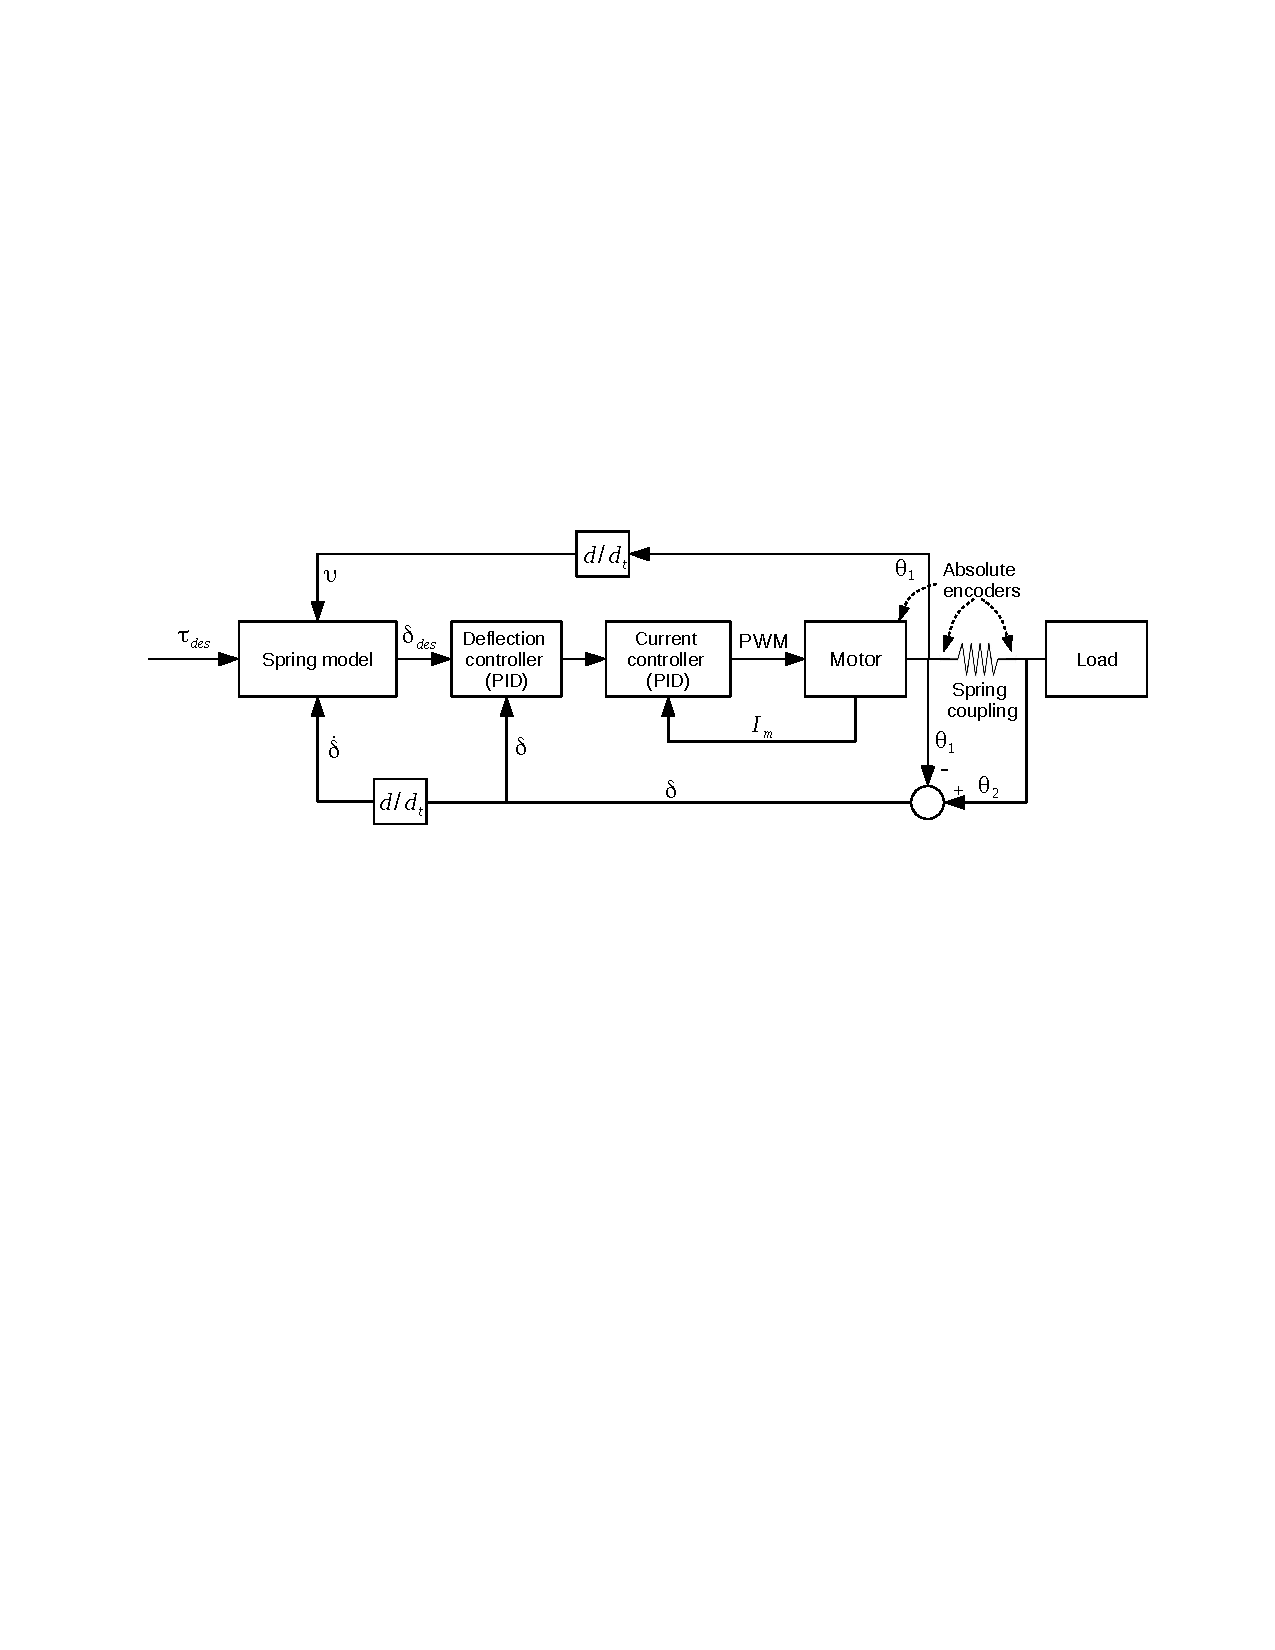
\includegraphics[width=1\textwidth, trim=2.5cm 13cm 2cm 8.5cm, clip]{images/torque_control_block_diagram.pdf}
    \caption{Complete actuator torque control scheme}
 \label{fig:controller_structure}
\end{figure}
%%%%%%%%%%%%%%%%%%%%%%%%%%%%%%%%%%%%%%%%%%%%%%%%%%%%%%%%%%%%%%%%%%%%%%%%%%%%%
The proposed torque control is verified in two torque tracking experiments. A chirp signal and a random-walk are given as the desired torques in these two experiments respectively (green lines) and the different controllers which are based on different spring models are evaluated in measured output torques (red and blue lines, see plot a,b of Fig.~\ref{fig:torque_tracking_result}). As can be seen from the comparison in tracking errors (see plot c,d), the torque control by using DGMM model presents better results than by using linear model in both experiments. Since the viscous friction of the system can not be compensated by the spring models completely, the performance of random-walk tracking (rmse=0.90) is better than chirp tracking (rmse=1.13), and the error of the chirp tracking is also raised slightly when the reference frequency is increased. 

%In the experiment of tracking a random-walk signal, since the output torque is controlled to follow step singals, the load approaches static when the given torque is constant. Therefore, the viscous friction which needs to be compensated is lower than that in the experiment of chirp tracking. As a consequence....
%%%%%%%%%%%%%%%%%%%%  Figure: torque tracking    %%%%%%%%%%%%%%%%%%%%%%%%%%%%
\begin{figure}[htb]
\centering
\advance\leftskip-1.1cm
\vspace*{-1.1 cm}
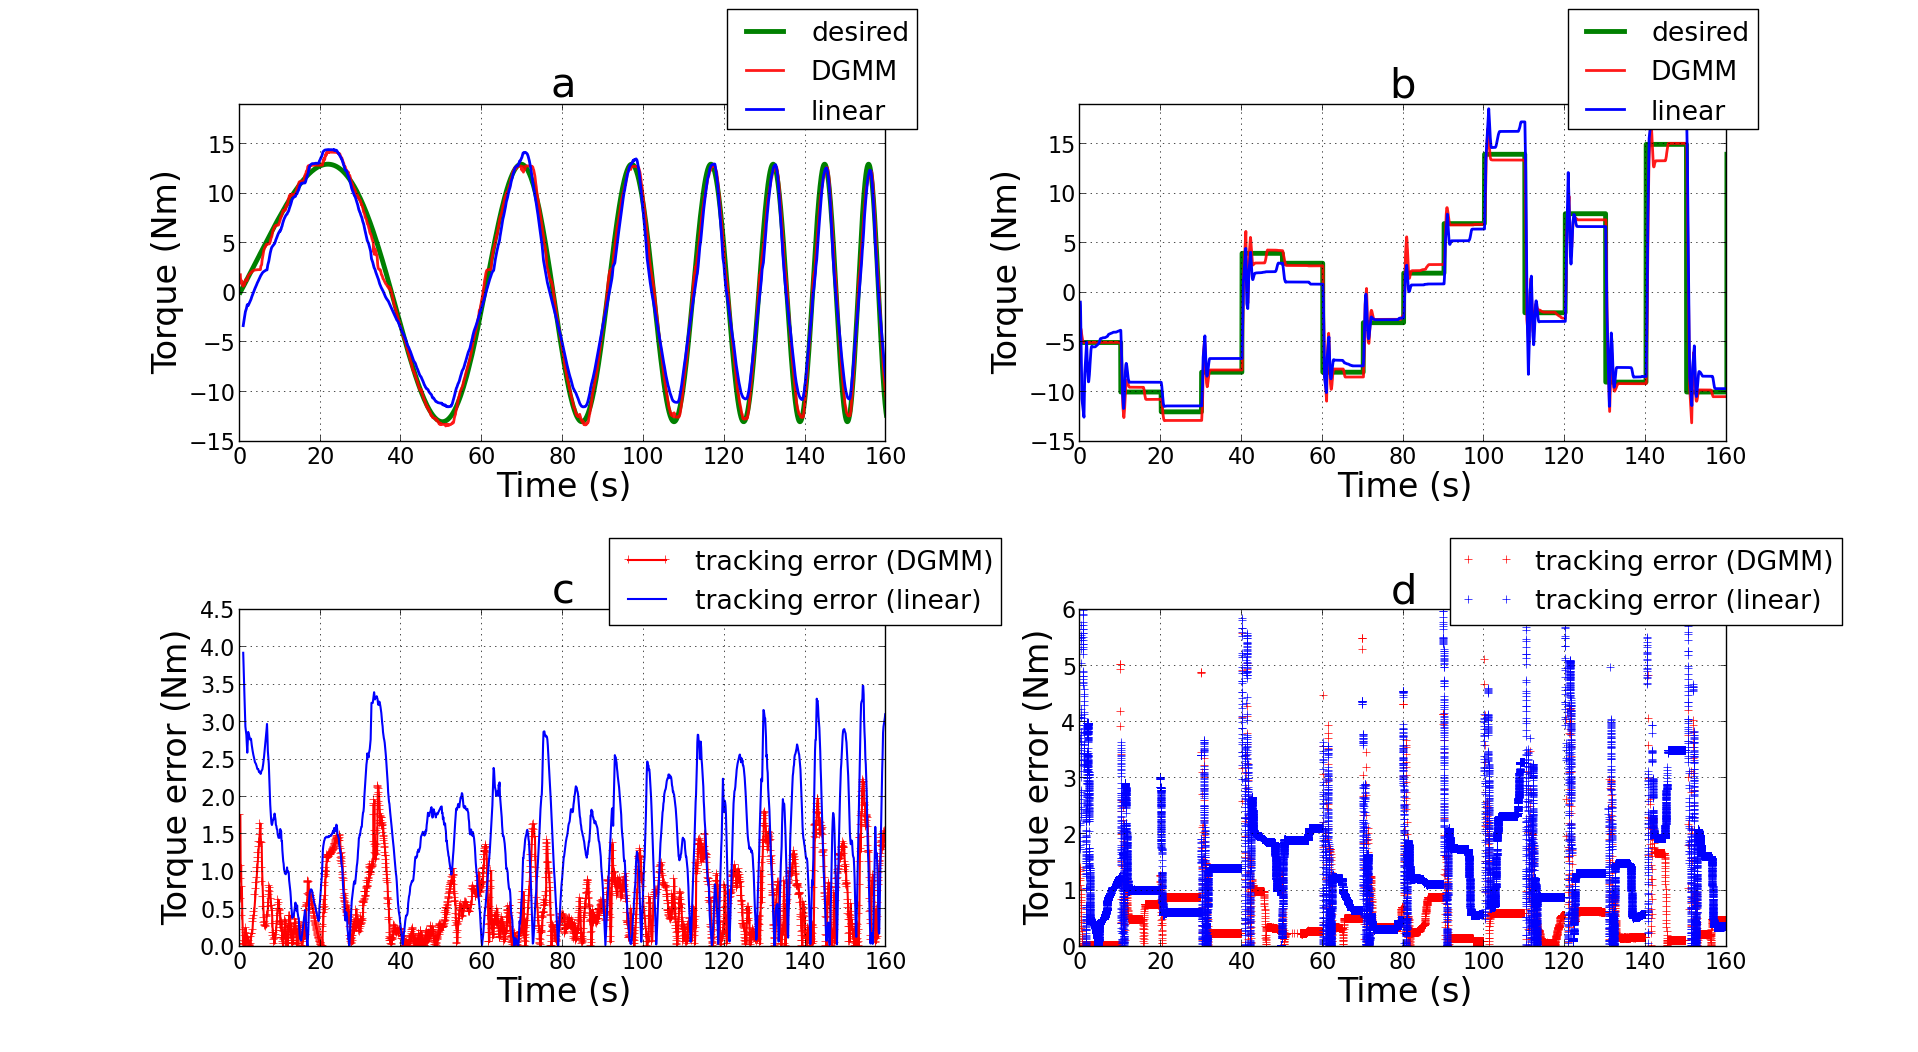
\includegraphics[width=1.15\columnwidth]{./images/4by3_torquetrack_chirp_rdwalk_comparison.png}
 \caption{\textit{a:} Result of the torque tracking with a chirp reference signal, \textit{b:} Result of the torque tracking with a random walk reference signal, \textit{c:} Torque tracking error with given chirp reference, \textit{d:} Torque tracking error with given random walk reference, }
 \label{fig:torque_tracking_result}
\end{figure}
%%%%%%%%%%%%%%%%%%%%%%%%%%%%%%%%%%%%%%%%%%%%%%%%%%%%%%%%%%%%%%%%%%%%%%%%%%%%%%






\iffalse
%%%%%%%%%%%%%%%%%%%%  Figure: torque tracking    %%%%%%%%%%%%%%%%%%%%%%%%%%%%
\begin{figure}[htb]
\centering
\advance\leftskip-1.1cm
\vspace*{-1.1 cm}
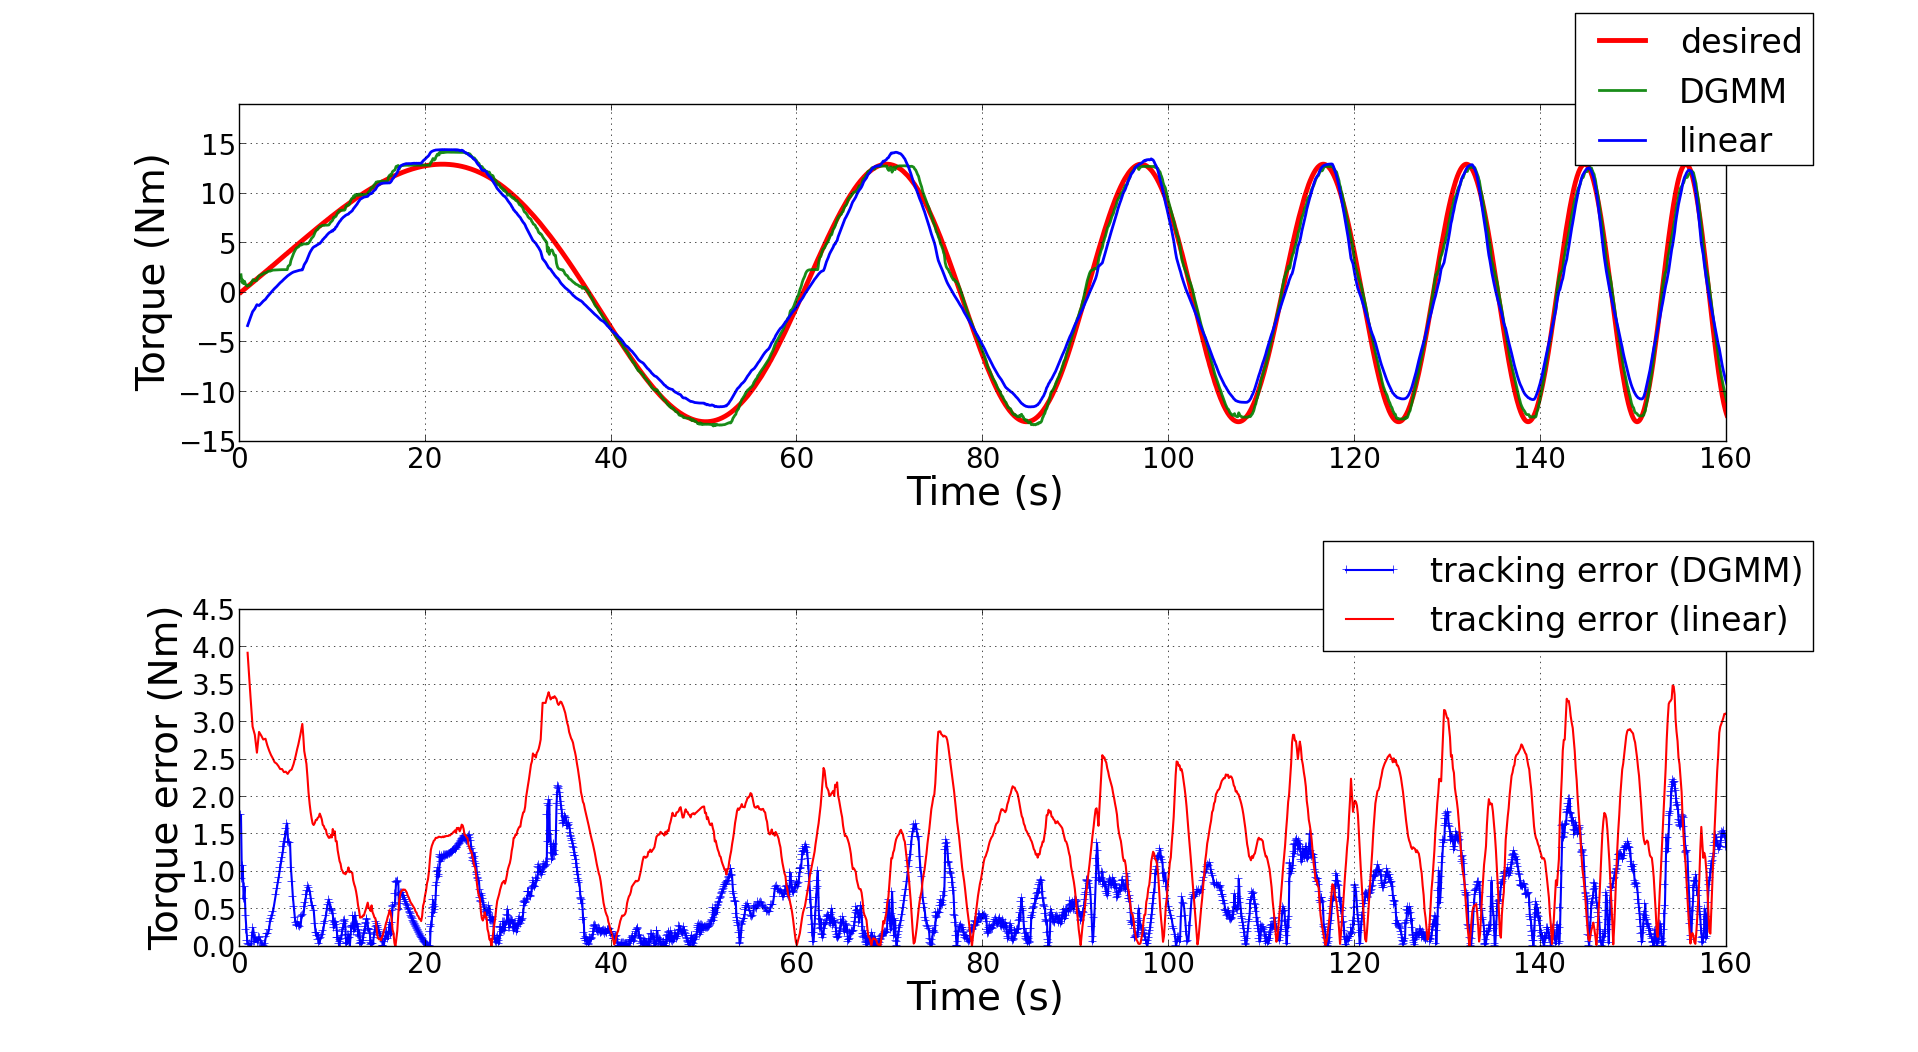
\includegraphics[width=1.15\columnwidth]{./images/4by3_dgmm_torquetrack_chirp_new.png}
 \caption{\textit{upper:} Result of the torque tracking with a chirp reference signal, \textit{lower:} Torque tracking error.}
 \label{fig:torque_tracking_result}
\end{figure}
%%%%%%%%%%%%%%%%%%%%%%%%%%%%%%%%%%%%%%%%%%%%%%%%%%%%%%%%%%%%%%%%%%%%%%%%%%%%%%

%%%%%%%%%%%%%%%%%%%%  Figure: torque tracking    %%%%%%%%%%%%%%%%%%%%%%%%%%%%
\begin{figure}[htb]
\centering
\advance\leftskip-1.1cm
\vspace*{-1.1 cm}
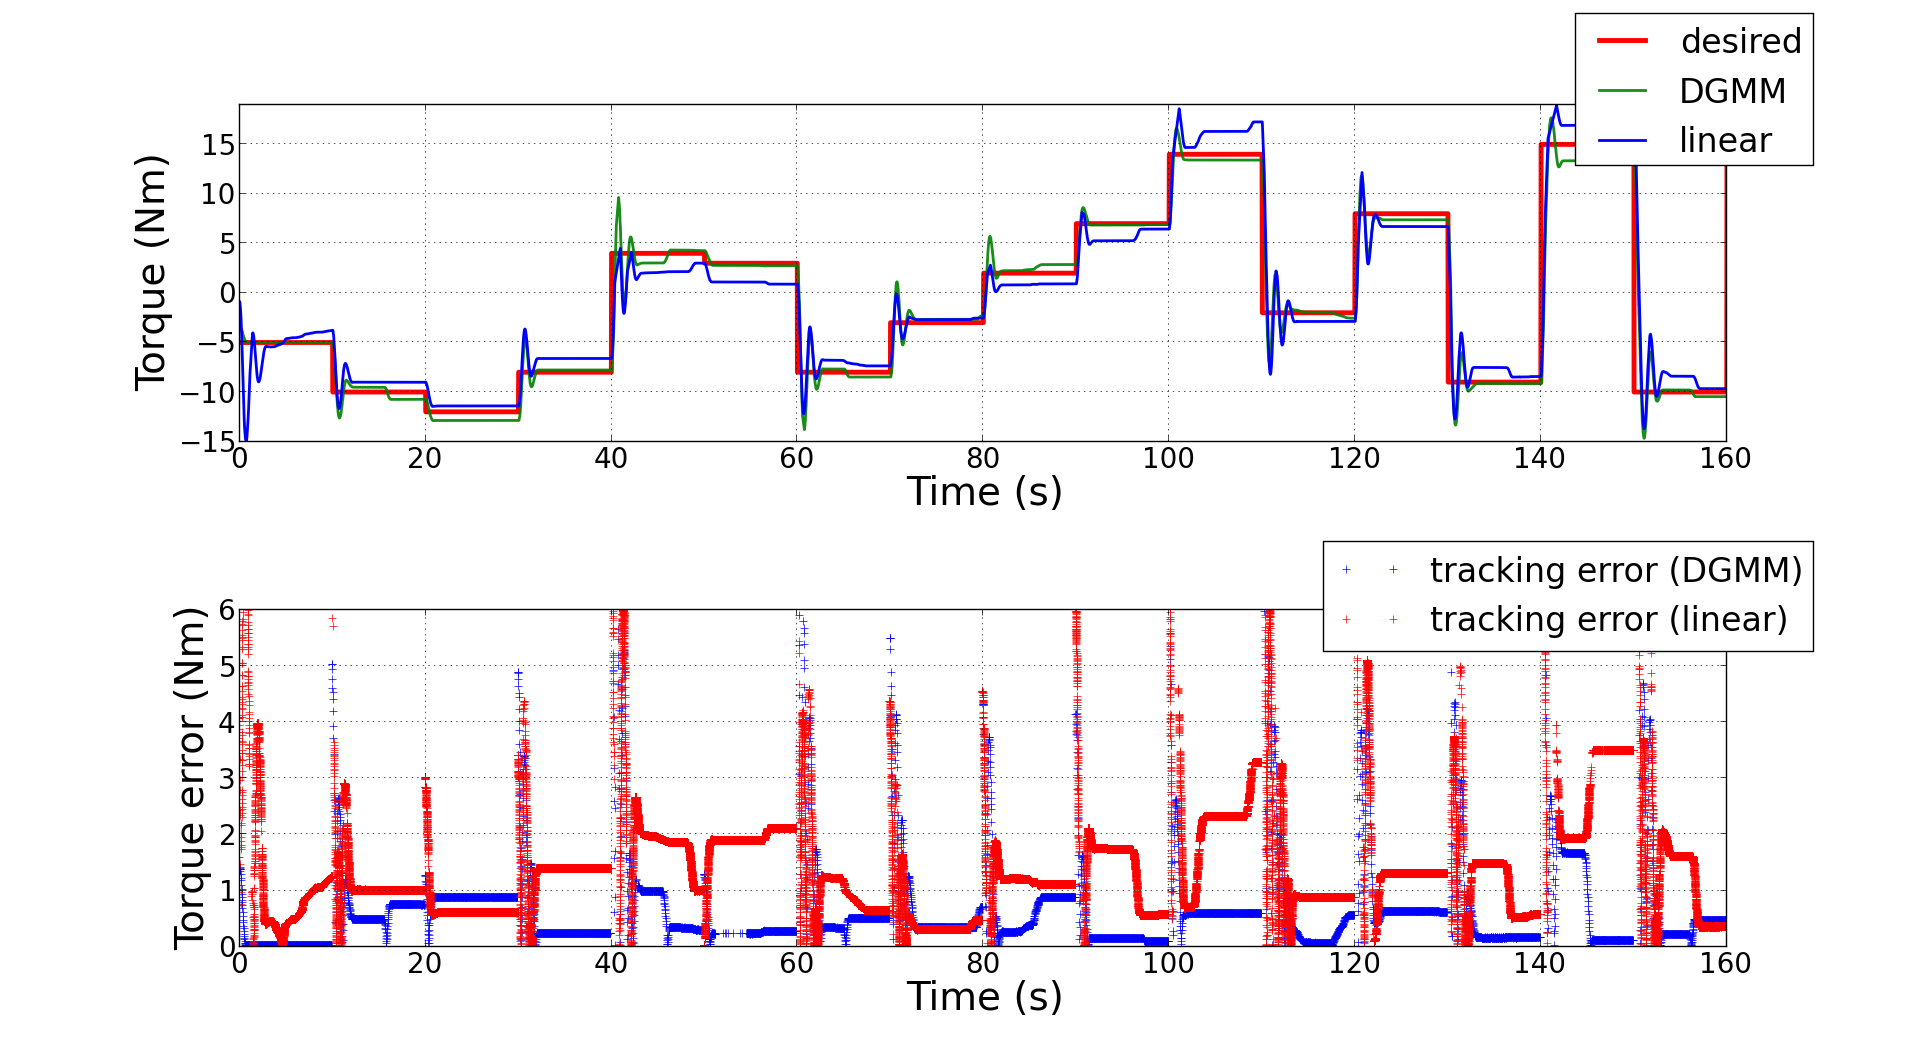
\includegraphics[width=1.15\columnwidth]{./images/4by3_dgmm_torquetrack_randomwalk_taumod.png}
 \caption{Result of torque tracking with a random-walk reference signal.}% \info{}}
 \label{fig:torque_tracking_result}
\end{figure}
%%%%%%%%%%%%%%%%%%%%%%%%%%%%%%%%%%%%%%%%%%%%%%%%%%%%%%%%%%%%%%%%%%%%%%%%%%%%%%
%Virtual Spring Element
%Gravity Compensation
%Zero Torque on Spring(Torque Control of High Compliant Series Elastic Actuator )
\fi
